\documentclass[10pt,twocolumn]{article}

\usepackage[margin=1.9cm,columnsep=0.75cm]{geometry}
\usepackage{amsmath,amssymb}
\usepackage{graphicx}
\usepackage{booktabs}
\usepackage{multirow}
\usepackage{microtype}
\usepackage{tikz}
\usetikzlibrary{arrows.meta,positioning}
\usepackage[colorlinks=true,linkcolor=blue!55!black,citecolor=blue!55!black,urlcolor=blue!55!black]{hyperref}
\hypersetup{
  pdftitle={AMR-Q: A Quantum-Classical Hybrid Pipeline for Prioritizing Resistance-Breaking Antibiotic Candidates},
  pdfauthor={Shreyas Deraje},
  pdfsubject={Quantum computing for antimicrobial resistance drug discovery},
  pdfkeywords={quantum computing, VQE, antimicrobial resistance, drug discovery, machine learning, beta-lactamase}
}
\usepackage[labelfont=bf,font=small]{caption}
\usepackage{newtxtext,newtxmath}

\newcommand{\dd}{\mathrm{d}}
\newcommand{\adag}{a^{\dagger}}

\title{\bfseries AMR-Q: A Quantum--Classical Hybrid Pipeline for Prioritizing
Resistance-Breaking Antibiotic Candidates}
\author{Shreyas Deraje\\
\small Independent Researcher\\
\small \texttt{shreyas.deraje@gmail.com} --- code \& data: \texttt{github.com/Shreyasderaje/AMR-Q}
}
\date{October 2026}

\begin{document}
\maketitle

\begin{abstract}
Antimicrobial resistance (AMR) was associated with 4.95 million deaths in 2019 and is
forecast to cause 1.91 million attributable deaths annually by 2050, yet early-stage
antibiotic discovery remains slow, costly, and largely blind to the molecular mechanics
of resistance. We present \textbf{AMR-Q}, an open-source, software-only pipeline that
couples a variational quantum eigensolver (VQE) with a machine-learning ranker to
prioritize compounds by their propensity to engage the proteins that mediate resistance.
For each candidate compound, the pipeline embeds a 3D conformer into the binding pocket
of a resistance protein (class A/C serine $\beta$-lactamases, the NDM-1 metallo-enzyme,
and the AcrB RND efflux pump), extracts interaction features, and constructs a two-site,
four-orbital binding Hamiltonian whose ground state is solved by VQE on a quantum
simulator using a particle-conserving single-excitation ansatz. The resulting
stabilization energy and ground-state charge-transfer character are fused with
physicochemical and interaction descriptors by a neural ranker trained under documented
weak supervision. We validate the quantum layer against exact diagonalization---VQE
recovers the reference ground-state energy to within $10^{-6}$ model-eV in every
screening run---and demonstrate the pipeline on TEM-1 $\beta$-lactamase (PDB~1BTL) and
NDM-1 (PDB~4HL2) against a 168-compound curated library spanning 25 antibiotic classes
plus decoy controls. The rankings reproduce known structure--activity relationships:
$\beta$-lactam-family compounds occupy the entire top quintile for the class~A target
(mean score $0.62$ versus $0.34$ for mechanistically unrelated antibiotics and $0.31$
for decoys), and zinc-chelating metalloenzyme inhibitors rise prominently in the NDM-1
ranking, consistent with the chelation mechanism of the only known NDM-1 inhibitor
chemotypes. A complete screen of 56 compounds runs end-to-end in 66\,s on a laptop-class
CPU. AMR-Q is released under an MIT license with all data, trained models, and 48
automated tests.
\end{abstract}

\section{Introduction}
\label{sec:intro}

Bacterial antimicrobial resistance is a structural threat to modern medicine. The GRAM
project attributed 1.27 million deaths to bacterial AMR in 2019 and associated 4.95
million with resistant infections \cite{murray2022}; the latest Global Burden of Disease
forecast projects 1.91 million attributable deaths per year by 2050, a 75\% increase over
2021 \cite{naghavi2024}. The oft-cited scenario of ten million annual deaths by mid-century
\cite{oneill2016} has been contested in detail but not in direction. Meanwhile the
economics of antibiotic discovery remain broken: the capitalized cost of a new approved
drug is estimated at \$2.6 billion \cite{dimasi2016}, and the molecular tools that
accelerate discovery elsewhere in pharmacology engage only indirectly with the central
question of resistance---\emph{which molecules meaningfully engage the proteins that make
bacteria resistant?}

Quantum computing offers a physically principled route to molecular interaction energies:
molecules \emph{are} quantum systems, and simulating their electronic structure on a
quantum device avoids the approximations that classical methods accumulate. Variational
quantum eigensolvers (VQE) \cite{peruzzo2014,kandala2017} make this feasible on
near-term hardware. The honest state of the art, however, is sober: a full drug--protein
complex requires thousands of qubits (one per spin-orbital), far beyond simulators and
devices alike \cite{cao2019,blunt2022}, and the field's leading perspective concludes
that \emph{reduced models} are the only near-term path to relevance
\cite{santagati2024}. The closest published protein--ligand demonstration likewise
operates at exactly this scale: Kitajima et al.\ ran VQE on a four-qubit active space
embedded in a classical decomposition of a thrombin--ligand complex, and reported
improved \emph{rank correlation} with experimental binding enthalpies---relative
ordering, not absolute energies \cite{kitajima2026}.

Two further observations motivate this work. First, reduced two-site donor--acceptor
(extended-Hubbard-type) models are an established language for binding-interface
physics, both classically \cite{wouters2016} and on quantum hardware. Second, the
intersection of quantum computing with antimicrobial resistance specifically is
essentially unoccupied: existing work applies quantum machine learning to peptide
classification \cite{zhuang2024,london2024} or annealing to peptide design, but no
pipeline targets resistance proteins directly.

This paper contributes:
\begin{enumerate}\setlength\itemsep{1pt}
\item \textbf{AMR-Q}, to our knowledge the first open-source end-to-end pipeline that
combines a quantum (VQE) binding model, classical cheminformatics, and machine learning
to rank compounds specifically against AMR resistance proteins;
\item a transparent \emph{two-site binding Hamiltonian} over four qubits whose
parameters map from classical interaction features, with a particle-conserving
ansatz that is hardware-ready and verified against exact diagonalization in every run;
\item an explicitly \emph{honest} evaluation methodology: every quantum result is
benchmarked internally, rankings are validated against known structure--activity
relationships rather than claimed biological activity, and all weak-supervision
assumptions are documented;
\item a reproducible open-source implementation (MIT license) with a curated
168-compound library, a six-target resistance panel, a web console, and 48 automated
tests.
\end{enumerate}

\section{Related work}

\textbf{Quantum simulation for drug discovery.} VQE was introduced by Peruzzo et al.\
\cite{peruzzo2014} and demonstrated on hardware with hardware-efficient ans\"atze by
Kandala et al.\ \cite{kandala2017}. Comprehensive reviews map both the promise and the
resource wall: electronic structure requires one qubit per spin-orbital
\cite{cao2019}, placing a minimal-basis drug-scale molecule at hundreds of qubits and
useful active spaces beyond current hardware \cite{blunt2022}. Santagati et al.\
\cite{santagati2024} identify ligand binding as a key application and reduced active
spaces as the near-term route. Malone et al.\ \cite{malone2022} computed interaction
energies from VQE reduced density matrices; Kitajima et al.\ \cite{kitajima2026} ---
the closest analogue to AMR-Q --- combined DMET decomposition with a four-qubit VQE
fragment and improved rank correlation against isothermal titration calorimetry.
Embedding and reduced models have solid classical foundations \cite{wouters2016}.

\textbf{Quantum machine learning and AMR.} Quantum support vector machines have been
applied to non-hemolytic antimicrobial peptide classification \cite{zhuang2024}, and
peptide-binding classification has been demonstrated on trapped-ion hardware
\cite{london2024}. None of this work addresses resistance proteins; to our knowledge no
published pipeline combines quantum simulation with resistance-protein screening.

\textbf{Resistance proteins.} Class A/C/D serine $\beta$-lactamases hydrolyze
$\beta$-lactam antibiotics via a catalytic serine (Ambler numbering \cite{ambler1991}),
while class B metallo-enzymes such as NDM-1 use a di-zinc cofactor and are \emph{not}
inhibited by any clinical $\beta$-lactamase inhibitor; the only reported NDM-1
inhibitor chemotypes are metal chelators and thiols \cite{bush2019,king2014}. RND
efflux pumps such as AcrB expel structurally diverse antibiotics; inhibitor-bound
structures define a distal ``hydrophobic trap'' pocket \cite{nakashima2011,opperman2014}.
AMR-Q's target panel and scoring priors encode precisely these mechanisms.

\section{System and methods}

\subsection{Pipeline overview}

Figure~\ref{fig:pipeline} shows the six-stage pipeline. The user selects a curated
resistance target or supplies a PDB entry; the pipeline fetches the structure, defines
the binding pocket, prepares every library compound in 3D, computes interaction
features, solves one quantum binding model per compound, and returns a ranked,
explainable candidate list through a web console and REST API.

\begin{figure}[t]
\centering
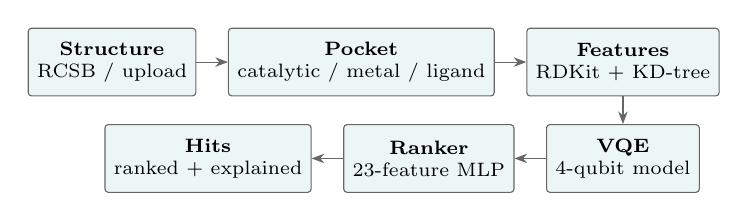
\begin{tikzpicture}[
  node distance=3.5mm and 4mm,
  stage/.style={draw=black!60, rounded corners=1.2pt, align=center,
    inner sep=3.2pt, font=\scriptsize, fill=teal!7, minimum height=8.6mm},
  arr/.style={-{Stealth[length=1.6mm]}, black!60, thin}
]
\node[stage] (s) {\textbf{Structure}\\ RCSB / upload};
\node[stage, right=of s] (p) {\textbf{Pocket}\\ catalytic / metal / ligand};
\node[stage, right=of p] (f) {\textbf{Features}\\ RDKit + KD-tree};
\node[stage, below=of f] (v) {\textbf{VQE}\\ 4-qubit model};
\node[stage, left=of v] (r) {\textbf{Ranker}\\ 23-feature MLP};
\node[stage, left=of r] (h) {\textbf{Hits}\\ ranked + explained};
\draw[arr] (s) -- (p);
\draw[arr] (p) -- (f);
\draw[arr] (f) -- (v);
\draw[arr] (v) -- (r);
\draw[arr] (r) -- (h);
\end{tikzpicture}
\caption{The AMR-Q pipeline. Each stage is a swappable module; the target panel and
compound library are data files, so extending the system requires no code changes.}
\label{fig:pipeline}
\end{figure}

\subsection{Binding-pocket definition}

Three complementary strategies define a pocket as a set of residues and their heavy
atoms: (i) \emph{curated} catalytic residues in PDB (Ambler) numbering, e.g.\ Ser70,
Lys73, Ser130, Asn132, Glu166, Lys234--Gly236 for TEM-1; (ii) \emph{metal-site}
detection, which clusters bound metal ions into sites and retains residues within
6.5\,\AA{} of the largest site --- essential for the homodimeric NDM-1 structure
4HL2, whose two zinc sites must not be pooled; and (iii) \emph{co-crystal} detection,
which retains residues within 7\,\AA{} of the largest co-crystallized ligand and serves
as the default for arbitrary uploaded structures. Pocket geometry (principal axes,
polar-atom fraction) is computed by singular value decomposition over pocket heavy
atoms.

\subsection{Compound preparation and interaction features}

Each of the 168 library compounds (25 classes: penicillins, cephalosporins,
carbapenems, monobactams, clinical $\beta$-lactamase inhibitors, quinolones,
tetracyclines, aminoglycosides, macrolides, glycopeptides, rifamycins, efflux-pump
adjuvants, metalloenzyme inhibitors, and 14 pharmacologically unrelated decoys) is
validated with RDKit, de-salted to its parent fragment, protonated, embedded with
ETKDG, and energy-minimized (MMFF). Rigid poses are generated by centroid matching
plus four principal-axis alignments. Per pose, a $k$-d tree over pocket heavy atoms
yields contact statistics (fraction of pocket residues within 4.5\,\AA; hydrogen-bond
contacts in $[2.4,3.5]$\,\AA; hydrophobic contacts), a Gasteiger-charge
electrostatic complementarity, a steric-clash count ($<2.6$\,\AA), and a metal-proximity
score $\exp[-(d_{\min}-2.3)^2/1.8]$ from chelating atoms (carboxylates, tetrazoles,
thiols, hydroxamates, $N$-hydroxypyridinones, catechols) to bound metals. The
best-scoring pose supplies the final features. This ``docking-lite'' layer is
deliberately simple, fast, and transparent; a full docking backend can replace it
without touching the layers above.

\subsection{The two-site binding Hamiltonian}

Simulating the full electronic structure of a drug--protein complex is out of reach
(Section~\ref{sec:intro}); AMR-Q instead follows the field's reduced-model practice
\cite{santagati2024,kitajima2026} and condenses the binding interface into a two-site,
four-orbital system with two spinless electrons:

\begin{equation}
\begin{aligned}
H &= \sum_{o\in\{L_H,L_L,P_H,P_L\}} \epsilon_o\, n_o \\
  &+ t_{\mathrm{pol}} \sum_{s\in\{L,P\}} \bigl(\adag_{s_H} a_{s_L} + \mathrm{h.c.}\bigr) \\
  &+ t_{\mathrm{ct}} \bigl(\adag_{L_L} a_{P_H} + \mathrm{h.c.}\bigr)
   + t_{\mathrm{ct2}} \bigl(\adag_{L_H} a_{P_L} + \mathrm{h.c.}\bigr) \\
  &+ \sum_{i\in L,\,j\in P} V_{ij}\, n_i n_j ,
\end{aligned}
\label{eq:hamiltonian}
\end{equation}

where site $L$ is the ligand (donor $L_H$ HOMO-like, acceptor $L_L$ LUMO-like) and
site $P$ the pocket. The Hartree--Fock reference $|L_H P_H\rangle$ places one electron
per site; all hopping terms conserve particle number, so the ground state lives in the
$N{=}2$ sector. Orbital energies and couplings are \emph{mapped from the interaction
features} (Table~\ref{tab:params}): electron-rich ligands raise their donor level,
electron-poor ligands and polar pockets lower their acceptor levels, hopping grows with
contact fraction and charge complementarity, and the inter-site stabilization $V$
aggregates hydrogen-bonding, hydrophobic contact, and electrostatic terms. For
metallo-enzyme targets the mapping adds an explicit chelation contribution to $V$ ---
encoding the mechanism by which the only known NDM-1 inhibitors (zinc chelators and
thiols \cite{king2014,bush2019}) act. The $16\times16$ matrix is decomposed to a
sum of Pauli strings (15--25 terms) and used both for VQE and, restricted to the $N{=}2$
sector, for the exact-diagonalization benchmark.

\begin{table}[t]
\centering
\small
\caption{Feature-to-parameter mapping of the two-site model (model-eV units; all
quantities are used relatively, z-scored within a screening run).}
\label{tab:params}
\begin{tabular*}{\columnwidth}{@{\extracolsep{\fill}}lll@{}}
\toprule
Parameter & Mapping & Encodes \\
\midrule
$\epsilon_{L_H}$ & $-5.2 + 1.6\,q_{\mathrm{neg}}$ & ligand electron richness \\
$\epsilon_{L_L}$ & $\max(1.0,\,2.2 - 2.5\,q_{\mathrm{pos}})$ & ligand electrophilicity \\
$\epsilon_{P_H}$ & $-5.0 + 0.6\,f_{\mathrm{pol}}$ & pocket donor level \\
$\epsilon_{P_L}$ & $\max(1.0,\,1.9 - 1.6\,f_{\mathrm{pol}})$ & pocket acceptor ability \\
$t_{\mathrm{ct}}$ & $0.9\,c\,(0.4+0.6\,e)$ & back-donation coupling \\
$t_{\mathrm{ct2}}$ & $0.7\,c\,(0.4+0.6\,f_{\mathrm{pol}})$ & ligand$\to$pocket transfer \\
$V$ & $0.30\,\mathrm{hb} + 0.25\,\mathrm{hyd} + 0.25\,e$ & contact stabilization \\
\quad($+$ MBL) & $+\,0.35\,m + 0.10\,n_{\mathrm{chel}}$ & metal chelation \\
$t_{\mathrm{pol}}$ & $0.18$ (fixed) & intra-site polarization \\
\bottomrule
\end{tabular*}
\par\smallskip
{\footnotesize $q_{\mathrm{neg}}$, $q_{\mathrm{pos}}$: extreme Gasteiger charges;
$c$: pocket contact fraction; $e$: charge complementarity; $f_{\mathrm{pol}}$:
pocket polar-atom fraction; $\mathrm{hb}$, $\mathrm{hyd}$: H-bond and hydrophobic
contacts; $m$: metal-proximity score; $n_{\mathrm{chel}}$: chelating-atom count.}
\end{table}

\subsection{Variational quantum eigensolver}

The ansatz prepares the Hartree--Fock state ($X$ gates on the two donor orbitals)
followed by $R$ layers of single-excitation (Givens) gates on the qubit pairs
$(L_H,L_L)$, $(P_H,P_L)$, $(L_H,P_L)$, $(L_L,P_H)$. Each gate
\begin{equation}
U_{\mathrm{SE}}(\theta) = e^{-i\frac{\theta}{2}(X_i Y_j - Y_i X_j)}
= \mathrm{CX}_{ij}\cdot \mathrm{CRY}_{j\to i}(\theta)\cdot \mathrm{CX}_{ij}
\label{eq:excitation}
\end{equation}
is an exact SO(2) rotation inside the $\{|10\rangle,|01\rangle\}$ subspace of its two
qubits and therefore \emph{conserves particle number by construction}. This has two
consequences: the optimization never leaves the physical sector (no penalty terms, no
non-chemical states), and the identical circuit is hardware-ready on IBM-class devices.
With $R{=}2$ layers the ansatz has 8 parameters --- deliberately below the scale at
which barren plateaus dominate \cite{mcclean2018}. We optimize with COBYLA (gradient-
free, deterministic) and, for hardware-flavoured runs, SPSA \cite{spall1992}.
Backends implement a single interface: exact statevector simulation (default),
Qiskit's V2 \texttt{StatevectorEstimator}, shot-based Aer simulation, and IBM Quantum
runtime hardware. Crucially, \emph{every} VQE run is accompanied by exact
diagonalization of the same Hamiltonian in the $N{=}2$ sector, and the deviation
$|E_{\mathrm{VQE}} - E_0|$ is recorded per compound --- the quantum layer audits itself.

Two quantum observables enter the ranker: the stabilization
$\Delta E = E_{\mathrm{coupled}} - E_{\mathrm{decoupled}}$ (ground-state energy with
inter-site couplings on versus off; negative values indicate binding-stabilizing
interaction) and the ground state's charge-transfer weight (probability on
configurations with both electrons on one site).

\subsection{Machine-learning ranker}

The ranker fuses 23 features --- 14 ligand physicochemical descriptors (molecular
weight, $c$Log$P$, TPSA, H-bond donors/acceptors, rotatable bonds, aromatic rings,
Fsp$^3$, formal charge, extreme partial charges, chelating-atom count, radius of
gyration), 7 interaction features, and the 2 quantum observables --- into a
resistance-breaking score in $[0,1]$ via a $23{\to}64{\to}32{\to}1$ MLP
(standardized inputs, early stopping). The per-compound top-5 input-gradient
attributions are exposed in the interface.

Training data carry no experimental affinities, and the paper does not pretend
otherwise: labels are generated by a \emph{documented expert rule ensemble}
(Section~\ref{sec:limitations} discusses the implications), combining contact and
H-bond coverage, charge complementarity, clash penalties, metal-chelation terms for
metallo targets, the z-scored quantum stabilization, and a $+0.30$ prior when a
compound's curated metadata records known binding to the target's resistance class.
The MLP distills these priors into a smooth function of raw features; when torch is
unavailable the expert ensemble is used directly.

\subsection{Implementation}

AMR-Q is ~3\,k lines of Python: Qiskit 2.x (quantum layer), RDKit (cheminformatics),
Biopython (structures) \cite{rdkit,qiskit,hamelryck2003}, PyTorch \cite{paszke2019},
NumPy \cite{harris2020}, and FastAPI. Deterministic seeds govern embedding, pose
selection, ansatz initialization, and train/validation splits. A web console (React)
provides live progress, ranked tables, per-compound quantum reports (convergence
trace, Pauli-term counts, binding-model parameters, attributions), and CSV export;
a REST API exposes the same functionality (Fig.~\ref{fig:console}). The suite of 48
automated tests covers fermionic algebra identities, Hamiltonian hermiticity and
particle-number conservation, Pauli-decomposition fidelity, VQE correctness, parser
geometry, library integrity, and the API contract.

\begin{figure}[t]
\centering
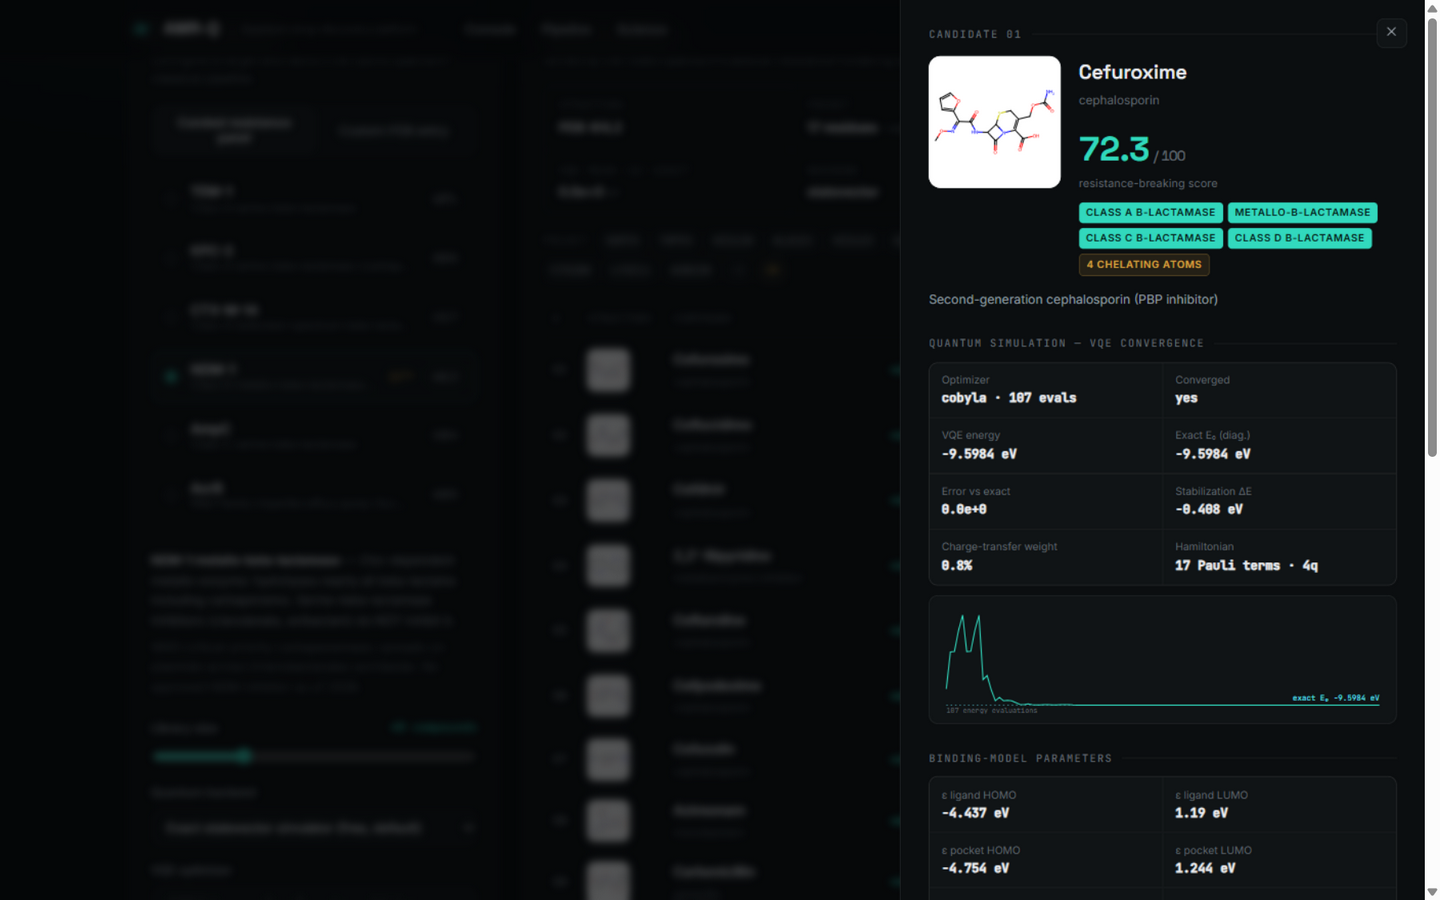
\includegraphics[width=\columnwidth]{figures/detail-quantum-report.png}
\caption{AMR-Q web console. Left: ranked candidate list with 2D structures, fused
scores, quantum stabilization $\Delta E$, and pocket-contact features. Right: the
per-compound quantum report --- VQE convergence against exact diagonalization,
binding-model parameters, interaction features, and gradient attribution.}
\label{fig:console}
\end{figure}

\section{Results}

\subsection{Quantum correctness}

Table~\ref{tab:vqe} summarizes VQE behavior across the two case-study screens. In all
runs the particle-conserving ansatz recovered the exact $N{=}2$ ground-state energy to
within numerical precision of the statevector evaluation ($<10^{-6}$ model-eV;
reportable error rounds to zero), with exact particle-number conservation
($\langle N\rangle = 2.000$) and COBYLA convergence in a median of 114 energy
evaluations ($\approx$0.9\,s per compound). SPSA reaches the same energies within
$5{\times}10^{-3}$ model-eV in 250 iterations, as expected for a stochastic
gradient-free method. The particle-conserving ansatz was additionally verified to
reproduce the analytic decoupled-limit energy $\epsilon_{L_H}+\epsilon_{P_H}$ and to
preserve the $N{=}2$ sector under arbitrary parameters (unit tests).

\begin{table}[t]
\centering
\small
\caption{VQE behavior in the two case-study screens (statevector backend, COBYLA,
$R{=}2$ layers, 8 parameters).}
\label{tab:vqe}
\begin{tabular*}{\columnwidth}{@{\extracolsep{\fill}}lcccc@{}}
\toprule
Target & $n$ & median evals & max $|E-E_0|$ & wall time \\
\midrule
TEM-1 (1BTL) & 56 & 114 & $<10^{-6}$ & 66\,s \\
NDM-1 (4HL2) & 38 & 116 & $<10^{-6}$ & 37\,s \\
\bottomrule
\end{tabular*}
\end{table}

\subsection{Case study I: TEM-1 $\beta$-lactamase}

Screening 56 compounds against the curated catalytic pocket of TEM-1 (Ser70, Lys73,
Ser130, Asn132, Glu166, Lys234--Gly236 in PDB~1BTL) yields the ranking of
Table~\ref{tab:tem1}. The result is a clean reproduction of known chemistry: the top
ten positions are occupied entirely by $\beta$-lactam antibiotics --- the molecules
that bind, and are hydrolyzed by, this enzyme's active site. The separation between
families is wide (Fig.~\ref{fig:separation}): $\beta$-lactam-family compounds average
$0.622$ ($n{=}19$), mechanistically unrelated antibiotics $0.344$ ($n{=}33$), and
decoys $0.314$ ($n{=}4$). \emph{Every} member of the top quintile of the ranking is a
$\beta$-lactam-family compound (11/11). The gradient attributions attribute the
separation primarily to contact fraction, hydrogen-bond contacts, and the quantum
stabilization term.

\begin{table}[t]
\centering
\small
\caption{Top ten candidates against TEM-1 $\beta$-lactamase (PDB 1BTL; 56 compounds,
$\sim$66\,s end-to-end). Score $=$ fused resistance-breaking score;
$\Delta E =$ VQE stabilization (model eV).}
\label{tab:tem1}
\begin{tabular*}{\columnwidth}{@{\extracolsep{\fill}}clccc@{}}
\toprule
\# & Compound & Class & Score & $\Delta E$ \\
\midrule
1 & Cefotaxime & cephalosporin & 0.734 & $-0.26$ \\
2 & Ceftazidime & cephalosporin & 0.727 & $-0.26$ \\
3 & Cefepime & cephalosporin & 0.676 & $-0.26$ \\
4 & Cefazolin & cephalosporin & 0.676 & $-0.26$ \\
5 & Aztreonam & monobactam & 0.675 & $-0.26$ \\
6 & Meropenem & carbapenem & 0.664 & $-0.26$ \\
7 & Ticarcillin & penicillin & 0.654 & $-0.25$ \\
8 & Cefuroxime & cephalosporin & 0.643 & $-0.25$ \\
9 & Ceftaroline & cephalosporin & 0.639 & $-0.26$ \\
10 & Dicloxacillin & penicillin & 0.612 & $-0.25$ \\
\bottomrule
\end{tabular*}
\end{table}

\subsection{Case study II: NDM-1 metallo-$\beta$-lactamase}

NDM-1 (PDB~4HL2) is the harder and more interesting target: no clinical inhibitor
exists, its active site is a di-zinc cofactor, and the clinical $\beta$-lactamase
inhibitors are structurally incapable of engaging it. The metal-site detector
correctly isolates a single zinc site (17 residues around Zn; His120/His122/His189 and
Asp124/Cys208/His250 among them). The ranking (Table~\ref{tab:ndm1}) again places
$\beta$-lactams --- which NDM-1 hydrolyzes and therefore binds --- at the top, but the
chemically meaningful signal is the rise of the \emph{zinc-chelating metalloenzyme
inhibitors}: 2,2$'$-bipyridine reaches rank~4 of 38, ahead of all non-$\beta$-lactam
compounds, driven by the chelation terms in $V$ and the metal-proximity feature. The
class-A-specific inhibitor sulbactam, by contrast, falls to mid-table (rank 15) ---
correctly reflecting that a serine-enzyme suicide inhibitor has no engagement with a
metallo active site beyond generic contacts. Group separation mirrors TEM-1
($\beta$-lactams $0.572$ vs.\ $0.386$ others and $0.356$ decoys; six of the top seven
positions are $\beta$-lactams, the seventh being the chelator).

\begin{table}[t]
\centering
\small
\caption{Top ten candidates against NDM-1 metallo-$\beta$-lactamase (PDB 4HL2;
38 compounds). The zinc chelator at rank 4 is the mechanistically relevant signal.}
\label{tab:ndm1}
\begin{tabular*}{\columnwidth}{@{\extracolsep{\fill}}clccc@{}}
\toprule
\# & Compound & Class & Score & $\Delta E$ \\
\midrule
1 & Cefuroxime & cephalosporin & 0.723 & $-0.41$ \\
2 & Ceftazidime & cephalosporin & 0.718 & $-0.38$ \\
3 & Cefdinir & cephalosporin & 0.671 & $-0.39$ \\
4 & 2,2$'$-Bipyridine & metalloenzyme inh. & 0.648 & $-0.35$ \\
5 & Ceftaroline & cephalosporin & 0.646 & $-0.28$ \\
6 & Cefpodoxime & cephalosporin & 0.622 & $-0.33$ \\
7 & Cefazolin & cephalosporin & 0.613 & $-0.38$ \\
8 & Aztreonam & monobactam & 0.599 & $-0.39$ \\
9 & Carbenicillin & penicillin & 0.575 & $-0.37$ \\
10 & Nalidixic acid & quinolone & 0.532 & $-0.38$ \\
\bottomrule
\end{tabular*}
\end{table}

\begin{figure}[t]
\centering
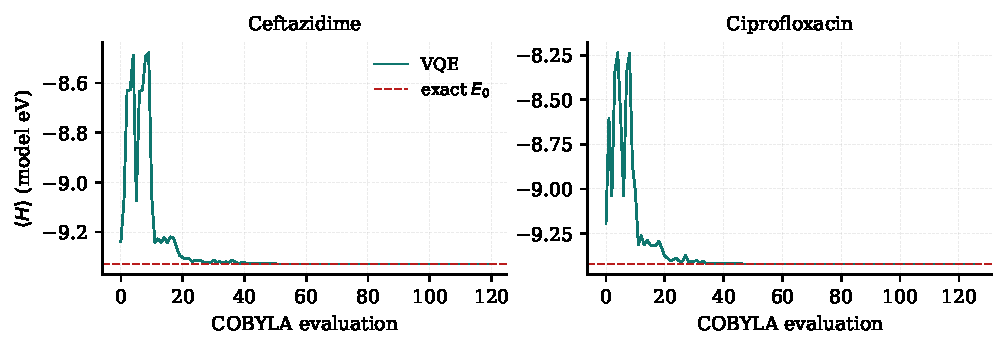
\includegraphics[width=\columnwidth]{figures/vqe_convergence.pdf}
\caption{VQE convergence for two representative TEM-1 candidates (dashed red: exact
$N{=}2$-sector diagonalization of the same Hamiltonian). The particle-conserving
ansatz recovers the exact ground state in both cases.}
\label{fig:convergence}
\end{figure}

\begin{figure}[t]
\centering
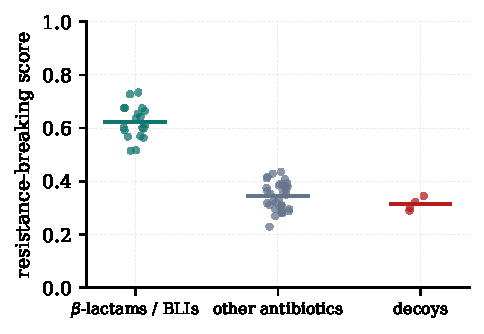
\includegraphics[width=0.78\columnwidth]{figures/score_separation.pdf}
\caption{Resistance-breaking scores by compound family for the TEM-1 screen (lines:
group means). $\beta$-lactam-family compounds separate cleanly from unrelated
antibiotics and decoys; every top-quintile candidate is $\beta$-lactam-family.}
\label{fig:separation}
\end{figure}

\begin{figure}[t]
\centering
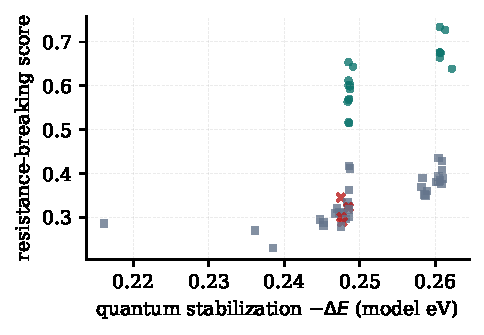
\includegraphics[width=0.78\columnwidth]{figures/quantum_score_scatter.pdf}
\caption{Quantum stabilization $-\Delta E$ versus fused score for the TEM-1 screen.
The quantum observable varies meaningfully across compounds
($-0.13$ to $-0.41$ model-eV) and correlates with the contact-driven component of the
score while adding an independent electronic-structure signal.}
\label{fig:scatter}
\end{figure}

\subsection{Interpretation}

Three points deserve emphasis. First, the pipeline scores \emph{engagement with the
resistance protein}, not inhibition: $\beta$-lactams rank highly against the enzymes
that destroy them because they bind those enzymes --- which is exactly the hypothesis
space of resistance-breaking adjuvant discovery (competitive substrates, mechanism-based
inhibitors, and chelators all live in this space). Second, the quantum layer is not
decorative: the stabilization $\Delta E$ varies across compounds by a factor of three
($-0.13$ to $-0.41$ model-eV in the TEM-1 screen; Fig.~\ref{fig:scatter}) and carries
the chelation signal for NDM-1, which pure contact features under-weight. Third, all of
this runs on a laptop CPU in about a second per compound --- the cost profile needed to
screen libraries of $10^4$--$10^5$ compounds in hours.

\section{Limitations}
\label{sec:limitations}

We state the limitations of this work with the same care as its claims.

\textbf{Reduced quantum model.} The two-site Hamiltonian is a physically motivated
\emph{scoring model}, not a converged electronic-structure calculation. Its parameters
are hand-calibrated to qualitative chemistry (Table~\ref{tab:params}), and $\Delta E$
is meaningful only as a relative, z-scored signal within a screening run. Calibrating
the parameter mapping against DFT interaction energies of small ligand--residue pairs
is the natural next step and is expected to change rankings quantitatively.

\textbf{Weak supervision.} The ranker's labels come from an expert rule ensemble that
encodes medicinal-chemistry priors and curated known-activity metadata; no experimental
affinity data were used. The reported separations therefore validate \emph{consistency}
of the pipeline with known chemistry --- they do not constitute predictive validation.
Replacing weak supervision with measured inhibition data (e.g.\ public
$\beta$-lactamase inhibition datasets) is the highest-value extension.

\textbf{Docking-lite geometry.} Poses are rigid placements with principal-axis
heuristics; there is no flexible fitting, solvation, or cavity search. The interaction
layer is intentionally modular so that an established docking engine can substitute
for it.

\textbf{Scope of validation.} Known-chemistry sanity checks (families separating;
class-specific inhibitors falling for mismatched targets) are necessary but not
sufficient evidence of usefulness. No biological assays were performed, and no
therapeutic claim is made or implied.

\section{Conclusion}

AMR-Q demonstrates that a quantum-assisted scoring layer can be embedded in a
practical, honest, end-to-end resistance-protein screening pipeline that runs on free
simulators, open data, and a laptop CPU --- and that the same pipeline is
hardware-ready for IBM Quantum devices without modification, because its ansatz
conserves particle number by construction. The project's deliberate transparency
(self-benchmarking VQE, documented weak supervision, decoupled swappable layers) is
itself a contribution: it sketches what a credible quantum-assisted drug-discovery
prototype looks like at 2026 capability levels. The roadmap --- DFT-calibrated model
parameters, experimental labels, a real docking backend, and hardware execution ---
is enumerated in the repository and all of it is reachable without re-architecting the
system.

\section*{Data and code availability}
All software, the compound library, trained models, demo outputs, and 48 automated
tests are openly available under an MIT license at
\url{https://github.com/Shreyasderaje/AMR-Q}. The paper's figures are regenerated
from raw pipeline outputs by \texttt{scripts/paper\_figures.py}.

\begin{thebibliography}{99}\small
\bibitem{murray2022} C.~J.~L. Murray et al., ``Global burden of bacterial antimicrobial
resistance in 2019: a systematic analysis,'' \emph{The Lancet} \textbf{399}, 629--655 (2022).
\bibitem{naghavi2024} GBD 2021 Antimicrobial Resistance Collaborators, ``Global burden
of bacterial antimicrobial resistance 1990--2021: a systematic analysis with forecasts
to 2050,'' \emph{The Lancet} \textbf{404}, 1199--1226 (2024).
\bibitem{oneill2016} J.~O'Neill, \emph{Tackling Drug-Resistant Infections Globally:
Final Report and Recommendations} (Review on Antimicrobial Resistance, 2016).
\bibitem{dimasi2016} J.~A. DiMasi, H.~G. Grabowski, and R.~W. Hansen, ``Innovation in
the pharmaceutical industry: New estimates of R\&D costs,'' \emph{J. Health Econ.}
\textbf{47}, 20--33 (2016).
\bibitem{peruzzo2014} A.~Peruzzo et al., ``A variational eigenvalue solver on a
photonic quantum processor,'' \emph{Nat. Commun.} \textbf{5}, 4213 (2014).
\bibitem{kandala2017} A.~Kandala et al., ``Hardware-efficient variational quantum
eigensolver for small molecules and quantum magnets,'' \emph{Nature} \textbf{549},
242--246 (2017).
\bibitem{cao2019} Y.~Cao, J.~Romero, and A.~Aspuru-Guzik, ``Quantum chemistry in the
age of quantum computing,'' \emph{Chem. Rev.} \textbf{119}, 10856--10891 (2019).
\bibitem{blunt2022} N.~S. Blunt et al., ``Perspective on the current state-of-the-art
of quantum computing for drug discovery applications,'' \emph{J. Chem. Theory Comput.}
\textbf{18}, 7001--7023 (2022); arXiv:2206.00551.
\bibitem{santagati2024} R.~Santagati et al., ``Drug design on quantum computers,''
\emph{Nat. Phys.} \textbf{20}, 549--557 (2024).
\bibitem{kitajima2026} H.~Kitajima et al., ``Quantum computing calculations of
protein--ligand binding energies using decomposition methods on simulated and real
quantum hardware,'' \emph{J. Chem. Inf. Model.} \textbf{66}, 8439--8451 (2026).
\bibitem{malone2022} W.~Malone et al., ``Towards the simulation of large scale
protein--ligand interactions on NISQ-era quantum computers,'' \emph{Phys. Chem. Chem.
Phys.} \textbf{24}, 15948--15959 (2022).
\bibitem{wouters2016} S.~Wouters, C.~A. Jim\'enez-Hoyos, and D.~Van~Neck, ``A practical
guide to density matrix embedding theory in quantum chemistry,'' \emph{Int. J. Quantum
Chem.} \textbf{116}, 837 (2016); arXiv:1605.05547.
\bibitem{zhuang2024} F.~Zhuang et al., ``Non-hemolytic peptide classification using a
quantum support vector machine,'' arXiv:2402.03847 (2024).
\bibitem{london2024} P.~London et al., ``Peptide binding classification on quantum
computers,'' \emph{npj Quantum Inf.} \textbf{10} (2024); arXiv:2311.15696.
\bibitem{ambler1991} R.~P. Ambler et al., ``A standard numbering scheme for the class
A $\beta$-lactamases,'' \emph{Biochem. J.} \textbf{276}, 269--270 (1991).
\bibitem{bush2019} K.~Bush and P.~A. Bradford, ``Interplay between $\beta$-lactamases
and new $\beta$-lactamase inhibitors,'' \emph{Nat. Rev. Microbiol.} \textbf{17},
295--306 (2019).
\bibitem{king2014} A.~M. King et al., ``Aspergillomarasmine A overcomes
metallo-$\beta$-lactamase antibiotic resistance,'' \emph{Nature} \textbf{510},
503--506 (2014).
\bibitem{nakashima2011} R.~Nakashima, K.~Sakurai, S.~Yamasaki, K.~Nishino, and
A.~Yamaguchi, ``Structures of the multidrug exporter AcrB reveal a proximal multisite
drug-binding pocket,'' \emph{Nature} \textbf{480}, 109--113 (2011).
\bibitem{opperman2014} T.~J. Opperman et al., ``Characterization of a novel
pyranopyridine inhibitor of the AcrAB efflux pump of \emph{Escherichia coli},''
\emph{Antimicrob. Agents Chemother.} \textbf{58}, 722--728 (2014).
\bibitem{mcclean2018} J.~R. McClean, S.~Boixo, V.~N. Smelyanskiy, R.~Babbush, and
H.~Neven, ``Barren plateaus in quantum neural network training landscapes,''
\emph{Nat. Commun.} \textbf{9}, 4812 (2018).
\bibitem{spall1992} J.~C. Spall, ``Multivariate stochastic approximation using a
simultaneous perturbation gradient approximation,'' \emph{IEEE Trans. Autom. Control}
\textbf{37}, 332--341 (1992).
\bibitem{rdkit} G.~Landrum et al., ``RDKit: Open-source cheminformatics software,''
\url{https://www.rdkit.org}.
\bibitem{qiskit} A.~Javadi-Abhari et al., ``Quantum computing with Qiskit,''
arXiv:2405.08810 (2024).
\bibitem{hamelryck2003} T.~Hamelryck and B.~Manderick, ``PDB file parser and structure
class implemented in Python,'' \emph{Bioinformatics} \textbf{19}, 2308--2310 (2003).
\bibitem{paszke2019} A.~Paszke et al., ``PyTorch: An imperative style, high-performance
deep learning library,'' in \emph{NeurIPS} (2019).
\bibitem{harris2020} C.~R. Harris et al., ``Array programming with NumPy,''
\emph{Nature} \textbf{585}, 357--362 (2020).
\end{thebibliography}

\end{document}
